%% grouprank.tex - Computing rank with limited nondeterminsm
%%
%% Copyright 2014, 2015 Jeffrey Finkelstein.
%%
%% This LaTeX markup document is made available under the terms of the Creative
%% Commons Attribution-ShareAlike 4.0 International License,
%% https://creativecommons.org/licenses/by-sa/4.0/.
\documentclass{article}

\usepackage{amsmath}
\usepackage{amssymb}
%% This must come before hyperref.
\usepackage{amsthm}
%% This is strongly recommended by biblatex.
\usepackage[english]{babel}
\usepackage[backend=biber]{biblatex}
\usepackage[T1]{fontenc}
%% This must come before csquotes.
\usepackage[utf8]{inputenc}
\usepackage{lmodern}
%% This is strongly recommended by biblatex.
\usepackage{csquotes}
%% This must come before hyperref.
\usepackage{thmtools}
%% This must come before complexity.
\usepackage{hyperref}
\usepackage{complexity}
\usepackage[firstpage]{draftwatermark}
\usepackage{microtype}
\usepackage{textcomp}
\usepackage{tikz}

\usetikzlibrary{trees}

\LoadMicrotypeFile{cmr}
\SetProtrusion
    [load=lmr-T1]
    {encoding=T1, family=lmr}
    {
      \textquotedblright = {,1000},
      \textquotedblleft = {1000,},
      {'} = {,1000},
      {,} = {,1000},
      {:} = {,1000},
      {;} = {,1000},
      {.} = {,1000}
    }


%% Set the ``work-in-progress'' watermark for the first page.
\SetWatermarkLightness{0.9}
\SetWatermarkText{Work-in-progress}
\SetWatermarkFontSize{3.5cm}

%% Set the title and author of the PDF file.
\hypersetup{pdftitle={Computing rank of finite algebraic structures with limited nondeterminism}, pdfauthor={Jeffrey Finkelstein}}

%% Declare the bibliography file.
\addbibresource{grouprank.bib}

%% Declare theorem-like environments.
\declaretheorem[numberwithin=section]{theorem}
\declaretheorem[numberlike=theorem,style=definition]{example}
\declaretheorem[numberlike=theorem]{lemma}
\declaretheorem[numberlike=theorem]{corollary}

%% Custom commands are declared here.
\newcommand{\email}[1]{\textlangle\href{mailto:#1}{\nolinkurl{#1}}\textrangle}
\newcommand{\todo}[1]{\textbf{TODO #1}}
\newcommand{\gen}[1]{\langle #1 \rangle}
\newcommand{\ceil}[1]{\lceil #1 \rceil}
\DeclareMathOperator{\cube}{cube}
\DeclareMathOperator{\rank}{rank}
\DeclareMathOperator{\Path}{Path}

%% Redefine the footnote environment so it has no reference and no number.
\long\def\symbolfootnote#1{\begingroup%
\def\thefootnote{\fnsymbol{footnote}}\footnotetext{#1}\endgroup}

%% Define the author, title, and date for the document.
\author{Jeffrey~Finkelstein\\ Computer Science Department, Boston University}
\title{Computing rank of finite algebraic structures \\ with limited nondeterminism}
%\date{\today}

\begin{document}

\maketitle

\symbolfootnote{%
  Copyright 2014, 2015 Jeffrey~Finkelstein \email{jeffreyf@bu.edu}.

  This document is licensed under the Creative Commons Attribution-ShareAlike 4.0 International License, which is available at \mbox{\url{https://creativecommons.org/licenses/by-sa/4.0/}}.
  The \LaTeX{} markup that generated this document can be downloaded from its website at \mbox{\url{https://github.com/jfinkels/grouprank}}.
  The markup is distributed under the same license.
}

\section{Introduction}

\todo{add information about complexity of the problem when the structures are provided as presentations instead of full Cayley tables}

\todo{show probability of success of a randomized reduction to (quasi)group membership}

An efficient algorithm computing the rank of a group (that is, the size of a minimum generating subset) benefits mathematicians, who use numerical algebra systems for research, cryptographers, who rely on algebraic systems for proofs of security, and theoretical computer scientists, who seek to understand which problems can be solved in a particular model of computation.
Before now, the best algorithm for computing the rank of a group required a polylogarithmic amount of space, which induces a superpolynomial (hence, inefficient) algorithm.
We reduced the best upper bound on the complexity of the group rank problem and provide a theoretically efficient algorithm for it.
This paper proves that with very short certificates of correctness, the group rank problem can be verified by highly restricted models of computation.

We prove that the problem of deciding whether the rank of a finite group, given as a Cayley table, is smaller than a specified number is decidable not only by a circuit of depth $O(\log \log n)$ augmented with $O(\log^2 n)$ nondeterministic bits, but also by a Turing machine using $O(\log n)$ space and $O(\log^2 n)$ bits of nondeterminism.
These models of computation are extremely limited in computational power, and the latter can be simulated by a deterministic Turing machine in polynomial time.
Using limited nondeterminism and restrictive models of computation as verifiers may also be useful in examining other algebraic problems.

The limited nondeterminism lens suggests some opportunities for further research in computational algebra.
Is computing the rank of a quasigroup, a problem more general than computing the rank of a group, in $\bL$ as well?
Is there a reduction between the problem of computing the rank of a quasigroup and the problem of deciding whether two quasigroups are isomorphism?
Finally, is the problem of computing a minimum generating sequence for a quasigroup strictly more difficult than the problem of computing the rank of a quasigroup?

\section{Preliminaries}

In this work, $\log n$ denotes the base two logarithm of $n$, for any natural number $n$.

\subsection{Complexity}

$\L$ is the class of languages decidable by a deterministic Turing machine that uses $O(\log n)$ space on inputs of length $n$.
$\L^2$ is the class of languages decidable by a deterministic Turing machine that uses $O(\log^2 n)$ space.
$\NL$ is the class of languages decidable by a nondeterministic Turing machine that uses $O(\log n)$ space.
$\bL$ is the subclass of $\NL$ in which the nondeterministic Turing machine uses at most $O(\log^2 n)$ nondeterministic bits.
$\FOLL$ is the class of languages decidable by a $\L$-uniform family of circuits with polynomial size, unbounded fan-in, and $O(\log \log n)$ depth.
$\bFOLL$ is the class of languages decidable by $\FOLL$ circuits that have been augmented with $O(\log^2 n)$ nondeterministic bits (gates with no inputs and one output).
$\AC_0$ and $\bAC_0$ are the restrictions of $\FOLL$ and $\bFOLL$, respectively, to depth $O(1)$.
In general, the class $\beta_2 \mathcal{C}$ is the class of languages decidable by $\mathcal{C}$ machines augmented with $O(\log^2 n)$ bits of nondeterminism.

If $L_1$ and $L_2$ are languages, there is a \emph{$\bAC_0$ conjunctive truth-table reduction} from $L_1$ to $L_2$, denoted $L_1 \leq^{\bAC_0}_{ctt} L_2$, if there is a function $f$ and a polynomial $p$ such that
\begin{itemize}
\item $f$ is computable in $\bAC_0$,
\item $f(x)$ outputs $(y_1, \dotsc, y_{p(n)})$ where $n$ is the length of $x$,
\item $x \in L_1$ if and only if $\bigwedge_{i = 1}^{p(n)} y_i \in L_2$.
\end{itemize}

\begin{lemma}\label{lem:ctt}
  Suppose $L_1$ and $L_2$ are languages and $L_1 \leq^{\bAC_0}_{ctt} L_2$.
  \begin{enumerate}
  \item If $L_2$ is in $\FOLL$, then $L_1$ is in $\bFOLL$.
  \item If $L_2$ is in $\L$, then $L_1$ is in $\bL$.
  \end{enumerate}
\end{lemma}
\begin{proof}
  Let $f$ be the $\bAC_0$ circuit computing the reduction and let $q$ be the polynomial bounding the length of its output.
  First, suppose $L_2$ is in $\FOLL$.
  Let $M_2$ be the $\FOLL$ circuit that decides $L_2$.
  To decide $L_1$, define the $\bFOLL$ circuit $M_1$ by
  \begin{equation*}
    M_1(x, w) = \bigwedge_{i = 1}^{q(n)} M_2(y_i),
  \end{equation*}
  where $|x| = n$ and $(y_1, \dotsc, y_{q(n)})$ is the output of $f(x, w)$.
  The depth of the $M_1$ circuit is dominated by the depth of $M_2$, which is $O(\log \log n)$.
  The number of nondeterministic bits required by $M_1$ is the same as the number of nondeterministic bits required by $f$, which is $O(\log^2 n)$.
  The circuit is polynomial in size because $f$ is polynomial in size, $M_2$ is polynomial in size, and there are a polynomial number of parallel instances of the circuit $M_2$.
  The correctness of the circuit follows from the correctness of $f$ and $M_2$.

  The proof is similar if $L_2$ is in $\L$.
  The only difference is that instead of a circuit computing the conjunction of $q(n)$ bits, we loop over each $y_i$ and check if each one causes $M_2$ to accept.
  Since there are a polynomial number of them, indexing them requires only logarithmic space.
  We also require the fact that logarithmic space computable functions compose.
\end{proof}

There is a \emph{$\NAC_0$ disjunctive truth-table reduction} from $L_1$ to $L_2$, denoted $L_1 \leq^{\NAC_0}_{dtt} L_2$, if there is a function $f$ and a polynomial $p$ such that
\begin{itemize}
\item $f$ is computable in $\NAC_0$,
\item $f(x)$ outputs $(y_1, \dotsc, y_{p(n)})$ where $n$ is the length of $x$,
\item $x \in L_1$ if and only if $\bigvee_{i = 1}^{p(n)} y_i \in L_2$.
\end{itemize}

\begin{lemma}\label{lem:dtt}
  Suppose $L_1$ and $L_2$ are languages and $L_1 \leq^{\NAC_0}_{dtt} L_2$.
  If $L_2$ is in $\NL$, then $L_1$ is in $\NL$.
\end{lemma}
\begin{proof}
  Let $f$ be the $\NAC_0$ circuit computing the reduction and let $q$ be the polynomial bounding the length of its output.
  Suppose $L_2$ is in $\NL$.
  Let $M_2$ be the nondeterministic Turing machine that decides $L_2$ with logarithmic space.
  To decide $L_1$, define the nondeterministic Turing machine $M_1$ as follows.
  On input $x$ of length $n$,
  \begin{enumerate}
  \item nondeterministically choose a binary string $w$ and a binary integer $i$ in $\{1, \dotsc, q(n)\}$,
  \item simulate $f(x, w)$ to produce $(y_1, \dotsc, y_{q(n)})$,
  \item accept if and only if $M_2(y_i)$ accepts.
  \end{enumerate}

  This machine requires only logarithmic space because it can simulate $f$ in logarithmic space and $M_2$ in logarithmic space (since functions computable in logarithmic space compose).
  The correctness of the machine follows from the correctness of $f$ and $M_2$.
\end{proof}

\subsection{Algebra}

An \emph{magma} is a set $G$ with a binary operation $\cdot$ that is closed on $G$.
Unless otherwise stated, we will only consider \emph{finite magmas}, in which $G$ is a finite set.
The \emph{Cayley table} of a magma with $n$ elements is the $n \times n$ table whose rows and columns are indexed by the elements of $G$ and where entry $(a, b)$ has value $c$ if $a \cdot b = c$.
If the binary operation is associative, the magma is called a \emph{semigroup}.
If the binary operation has the property that for each $a$ and $b$ in $G$ there are unique elements $x$ and $y$ in $G$ such that $a \cdot x = b$ and $y \cdot a = b$, the magma is called a \emph{quasigroup}.
(In other words, each quasigroup element appears exactly once in each row and each column of the Cayley table of $G$, or the Cayley table is a \emph{Latin square}.)
If a quasigroup is nonempty and associative, then it is a \emph{group}.
Alternately, if a semigroup has an identity and inverses, then it is a group.
%% Thus if a magma is nonempty, a semigroup, and a quasigroup, it is a group.

\begin{example}\label{ex:quasigroup}
  The smallest nonempty quasigroup that is not also a group has three elements, $\{a, b, c\}$.
  Its Cayley table is
  \begin{equation*}
    \begin{array}{c | c c c}
      \cdot & a & b & c \\
      \hline
      a & a & b & c \\
      b & c & a & b \\
      c & b & c & a \\
    \end{array}
  \end{equation*}
  Examining the table reveals that there is exactly one of each quasigroup element in each row and column.
  This quasigroup is not associative because $b \cdot (a \cdot b) = b \cdot b = a$ but $(b \cdot a) \cdot b = c \cdot b = c$.
  Also, it has a left identity, $a$, but no right identity.
\end{example}

\begin{example}
  The \emph{right zero semigroup} is the semigroup in which each element is a right zero.
  Its Cayley table is
  \begin{equation*}
    \begin{array}{c | c c c}
      \cdot & a & b & c \\
      \hline
      a & a & b & c \\
      b & a & b & c \\
      c & a & b & c \\
    \end{array}
  \end{equation*}
  The associativity of this semigroup can be determined by examining all possible triples $(x, y, z)$ in $G^3$ and checking that $(x \cdot y) \cdot z = x \cdot (y \cdot z)$.
  Each element of this semigroup is a left identity and a right zero, but there are no right identities, so it is not a group.

  Unlike for the Latin square property in the previous example, there is no obvious way to tell whether a binary operation is associative simply by scanning the rows and columns.
  In other words, given only its Cayley table, determining whether a magma is a quasigroup \emph{seems} easier than determining whether a magma is a semigroup.
  However, there is a polynomial time algorithm, attributed to F.~W.~Light, for deciding whether a magma is associative; it is simply the naïve algorithmic implementation of the associativity condition.
\end{example}

\begin{example}
  There is a unique (up to isomorphism) group on three elements $\{a, b, c\}$.
  Its Cayley table is
  \begin{equation*}
    \begin{array}{c | c c c}
      \cdot & a & b & c \\
      \hline
      a & a & b & c \\
      b & b & c & a \\
      c & c & a & b \\
    \end{array}
  \end{equation*}
  This is both a semigroup and a quasigroup.
\end{example}

A \emph{parenthesization} $P$ of a sequence of quasigroup elements $(g_0, \dotsc, g_k)$ is a binary tree that has the quasigroup elements as its leaves (in the order indicated by the sequence).
The \emph{parenthesized product} of a sequence of quasigroup elements $(g_0, \dotsc, g_k)$ with parenthesization $P$, denoted $P(g_0, \dotsc, g_k)$, is the quasigroup element that results from performing the quasigroup product in the order indicated by the parenthesization.

\begin{example}
  Consider $(a, c, a, b)$, a sequence of four elements from the quasigroup defined in \autoref{ex:quasigroup}.
  One parenthesization of this sequence is
  \begin{equation*}
    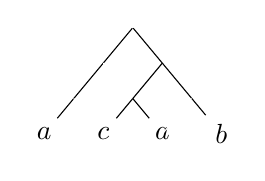
\begin{tikzpicture}[xscale=0.5, yscale=0.3]
      \node[minimum size=0pt, inner sep=0pt] {}
      child {
        child {
          child {node {$a$}}
          child[color=white] {}
        }
        child[color=white] {}
      }
      child {
        child {
          child {node {$c$}}
          child {node {$a$}}
        }
        child {
          child[color=white] {}
          child {node {$b$}}
        }
      };
    \end{tikzpicture}
  \end{equation*}
  which corresponds to the parenthesized product $a \cdot ((c \cdot a) \cdot b)$.
  According to the Cayley table, this product equals $a$.
\end{example}

If $(g_0, \dotsc, g_k)$ is a finite sequence of quasigroup elements denoted $S$ and $P$ is a parenthesization of that sequence, then the \emph{cube of $S$ with respect to $P$}, denoted $\cube_P(S)$, is defined
\begin{equation*}
  \cube_P(S) = \left\{P(g_0, g_1^{\epsilon_1}, \dotsc, g_k^{\epsilon_k}) \, \middle| \, \epsilon_i \in \{0, 1\} \text{ for each } i \right\}.
\end{equation*}
(This is called a ``cube'' because each vertex of the $k$-dimensional Boolean hypercube, when interpreted as a binary string $\epsilon_1 \dotsb \epsilon_k$, yields a quasigroup element.)
If $\cube_P(G) = G$, then $g$ is called a \emph{cube generating sequence of size $k + 1$} for the quasigroup $G$.
The \emph{rank of a quasigroup $G$}, denoted $\rank(G)$, is the minimum size of a cube generating sequence.
\footnote{
  This is a nonstandard definition of ``rank'' for quasigroups.
  Elsewhere, the rank of a quasigroup is the number of blocks in the partition of the quasigroup into conjugacy classes according to the action of the quasigroup on itself.
}

\begin{example}
  \todo{Example of a cube generating sequence for a quasigroup.}
\end{example}

If $G$ is a semigroup, the operation is associative, so the parenthesization is superfluous (that is, for any parenthesization $P$ and any sequence $(g_0, \dotsc, g_k)$, we have $P(g_0, \dotsc, g_k) = g_0 \cdot \dotsb \cdot g_k$).
If $S$ is a subset of semigroup elements, the \emph{subsemigroup generated by $S$}, denoted $\gen{S}$, is the closure of $S$ under the group operation.
If $\gen{S} = G$, then $S$ is called a \emph{generating set for $G$}.
The \emph{rank of a semigroup $G$}, denoted $\rank(G)$, is the minimum cardinality of a generating set.
Contrast the rank of a semigroup with the rank of a quasigroup: the former is the size of a set, the latter the size of a sequence.

If $G$ is a group, then it is a semigroup (and a quasigroup) so the same definitions and terminology apply.

\begin{example}
  Consider the elementary abelian $2$-group, $(\mathbb{Z} / 2 \mathbb{Z})^k$, for some positive integer $k$.
  Let $n$ denote the order of this group, so $n = 2^k$.
  The minimum generating set for this group is $\{e_1, \dotsc, e_k\}$, where $e_i$ is the $k$-tuple with a one in the $i$th position and a zero in each other position.
  Thus the group has a minimum generating set of size $k$, which is $\log n$.
\end{example}

Quasigroups have small cube generating sequences, and groups have small generating sets.
As of this publication, upper bounds on the size of generating sets for semigroups remain the subject of research \autocite{gray14}.
An upper bound for quasigroups can be proven by the probabilistic method, and an upper bound for groups can be proven inductively considering cosets of increasing size.

\todo{use probabilistic method to show existence of a short generating set for semigroups?}

\todo{for semigroups, it seems the rank can be computed from the complicated formulas in \autocite{gray14}; what upper bound does this give for arbitrary finite semigroups?}

\begin{lemma}[{\autocite[Theorem~3.3]{ctw13}}]\label{lem:small}
  Each finite quasigroup with $n$ elements has a cube generating sequence of size $O(\log n)$ with a parenthesization of depth $O(\log \log n)$.
\end{lemma}

\begin{lemma}\label{lem:log}
  If $G$ is a finite group of order $n$ then the minimum size of a generating set is at most $\log n$, with equality when the group is a finite elementary abelian $2$-group.
\end{lemma}
\todo{Should I include the proof here?}
%% %% This proof is from \url{http://www.imsc.res.in/~arvind/notes.pdf}.
%% \begin{proof}
%%   Suppose $m$ is the size of the minimum generating set.
%%   Let $H_0 = \gen{e}$, where $e$ is the identity element in $G$.
%%   For each $i \in \{1, \dotsc, m\}$, let $H_i = \gen{H_{i - 1}, x_i}$ where $x_i \in (G \setminus H_{i - 1})$.
%%   Such an $x_i$ must exist for each $i$ because otherwise we would have some set $H_j$, of size less than $m$, which generates the group $G$; this violates the hypothesis that $m$ is the minimum size of a generating set for $G$.

%%   Now, for each $i \in \{1, \dotsc, m\}$, we have $x_i \neq e$, by construction.
%%   Furthermore, the cosets $x_i \gen{H_{i - 1}}$ and $e \gen{H_{i - 1}}$ are disjoint.
%%   If we suppose to the contrary that there is some element $y \in e \gen{H_{i - 1}} \cap x_i \gen{H_{i - 1}}$, then $y = x_i h$ for some $h \in H_{i - 1}$, which implies $x_i = yh^{-1}$, and hence $x_i \in H_{i - 1}$ since both $y$ and $h$ are in $H_{i - 1}$.
%%   This is a contradiction with the hypothesis that $x_i \in (G \setminus H_{i - 1})$.
%%   Therefore $|H_i| \geq 2 |H_{i - 1}|$.
%%   By induction, $|G| = |H_m| \geq 2^m$, which implies $m \leq \log |G| = \log n$.
%% \end{proof}

\section{Efficient computation of membership}

\todo{Introduction and summary paragraph here.}

The \textsc{Cube Membership} problem is defined as follows.
The inputs are a quasigroup $G$ given as a Cayley table, a quasigroup element $h$, a finite sequence of quasigroup elements $S$, and a parenthesization $P$ for that sequence.
The problem is to decide whether $h \in \cube_P(S)$.

How does a circuit access a Cayley table for a quasigroup of order $n$?
\footnote{This work avoids representing problems using first-order logic, as in the original definition of $\FOLL$ from \autocite{bklm01}, though the logic definition may provide a more natural representation of this sort of information.}
One way for a circuit to compute the product of two quasigroup elements using the Cayley table is via a multiplexer.
In the multiplexer, each input has $O(\log n)$ bits, since each quasigroup element can be represented with $O(\log n)$ bits and each input is a pair of quasigroup elements.
A multiplexer that selects from $n^2$ inputs, each of length $O(\log n)$, can be implemented by an \emph{unbounded fan-in} circuit of depth $O(1)$ and size $O(n^2 \log n)$.

\begin{lemma}[{Implicit in \autocite[Theorem~3.4]{ctw13}}]\label{lem:cubemem}
  \textsc{Cube Membership} is decidable by an $\L$-uniform family of unbounded fan-in circuits with size $O(2^k k n^2 \log n)$ and depth $O(d)$, where $n$ is the order of the quasigroup, $k$ is the size of the generating sequence, and $d$ is the depth of the parenthesization.

  In particular, if $k$ is in $O(\log n)$ and $d$ is in $O(\log \log n)$, then the circuit is of size polynomial in $n$ and of depth $O(\log \log n)$.
\end{lemma}
\begin{proof}
  The input to the circuit is the Cayley table for a quasigroup, a quasigroup element $h$, a generating sequence $S$, and a parenthesization $P$.
  Suppose $S = (g_0, \dotsc, g_k)$ for some positive integer $k$.
  Since the circuit needs to determine if $h$ is in $\cube_P(S)$, the circuit accepts if and only if there is some sequence of bits $(\epsilon_1, \dotsc, \epsilon_k)$ such that $h = P(g_0, g_1^{\epsilon_1}, \dotsc, g_k^{\epsilon_k})$.
  Thus the circuit consists of $2^k$ subcircuits joined to a single \textsc{or} gate, each subcircuit deciding whether one of the $2^k$ possible $k$-bit sequences $(\epsilon_1, \dotsc, \epsilon_k)$ produces $h$ under the given parenthesization.

  The subcircuit corresponding to binary sequence $(\epsilon_1, \dotsc, \epsilon_k)$ computes the parenthesized product $P(g_0, g_1^{\epsilon_1}, \dotsc, g_k^{\epsilon_k})$.
  Computing the product of two quasigroup elements can be implemented in $O(n^2 \log n)$ size and $O(1)$ depth, as described in the paragraph preceding this lemma.
  Computing the parenthesized product therefore can be implemented in $O(k n^2 \log n)$ size and $O(d)$ depth, where $d$ is the depth of the parenthesization.
  Comparing the element produced this way to the element $h$ can be done with a constant depth, $O(\log n)$ size equality comparison circuit.

  We conclude that the overall size of the circuit is $O(2^k k n^2 \log n)$ and the overall depth of the circuit is $O(d)$.
\end{proof}

\todo{define semigroups}
The \textsc{Subsemigroup Membership} problem is defined as follows.
The inputs are a semigroup $G$ given as a Cayley table, a semigroup element $h$, and a finite set $S$ of semigroup elements.
The problem is to decide whether $h \in \gen{S}$.

\todo{Is there a cleverer way of computing subsemigroup membership faster than simply solving st-connectivity?}

\begin{lemma}\label{lem:subsemigroupmem}
  \textsc{Subsemigroup Membership} is in $\NL$.
\end{lemma}
\begin{proof}
  We will show a logarithmic space disjunctive truth-table reduction from \textsc{Subsemigroup Membership} to \textsc{Directed Path}.
  Since the latter problem is in $\NL$ and $\NL$ is closed under this type of reduction, we conclude that the former problem is in $\NL$ as well.

  Suppose $G$ is the semigroup, $h$ is the semigroup element, and $S$ is the set of subsemigroup generators described in the problem definition.
  The Cayley table induces an edge-labeled directed multigraph $\Gamma$ with self-loops: the vertices of the graph are the semigroup elements, and for each semigroup element $a$, $b$, and $c$, there is an edge labeled $b$ from $a$ to $c$ if $a \cdot b = c$.
  Consider the subgraph $\Gamma_S$ induced by those edges whose labels are in $S$.
  The element $h$ is in $\gen{S}$ if and only if there is a path from some vertex in $S$ to $h$.
  In other words, if $S = \{s_1, \dotsc, s_m\}$ for some natural number $m$ and $\Path(\Gamma_S, h, s_i)$ is a proposition that is true exactly when there is a directed path from $h$ to $s_i$ in $\Gamma_S$,
  \begin{equation*}
    h \in \gen{S} \iff \bigvee_{i = 1}^m \Path(\Gamma_S, h, s_i).
  \end{equation*}
  Therefore we choose the reduction to be $(G, h, S) \mapsto ((\Gamma_S, h, s_1), \dotsc, (\Gamma_S, h, s_m))$.

  Computing the adjacency matrix of $\Gamma_S$ from the Cayley table of $G$ and the set $S$ can be done in logarithmic space by setting each entry $(x, y)$ in the Cayley table to be zero if $y$ is not in $S$.
  Iterating over all edges in the adjacency matrix requires logarithmic space, and enumerating each of the $m$ outputs requires space logarithmic in $m$, which is logarithmic in $n$ because $m \leq n$.
  We conclude that the reduction is a correct logarithmic space disjunctive truth-table reduction.
\end{proof}

The \textsc{Subgroup Membership} problem is defined as follows.
The inputs are a group $G$ given as a Cayley table, a group element $h$, and a finite set $S$ of group elements.
The problem is to decide whether $h \in \gen{S}$.

\begin{lemma}\label{lem:subgroupmem}
  \textsc{Subgroup Membership} is in $\L$.
\end{lemma}
\begin{proof}
  The problem is in $\SL$ by a reduction to \textsc{Undirected Path} \autocite[Section~3]{bm89}, and $\SL = \L$ \cite{reingold08}.
\end{proof}

\section{Efficient computation of rank}

\todo{foreword and summary here}

The \textsc{Quasigroup Rank} problem is defined as follows.
Given the Cayley table of a quasigroup and an integer $k$ in binary, decide whether the rank of the quasigroup is $k$ or less.
The \textsc{Group Rank} problem is defined similarly.

The \textsc{Quasigroup Isomorphism} problem is the problem of determining whether there is a bijection between two quasigroups (again, given as Cayley tables) that preserves the quasigroup operation.
This problem is in $\bFOLL$ \autocite[Theorem~3.4]{ctw13}.
Implicit in that algorithm is the following reduction.

\begin{lemma}\label{lem:ranktomem}
  \mbox{}
  \begin{enumerate}
  \item $\textsc{Semigroup Rank} \leq^{\NAC_0}_{ctt} \textsc{Subsemigroup Membership}$.
    \todo{define semigroup rank}
  \item $\textsc{Quasigroup Rank} \leq^{\bAC_0}_{ctt} \textsc{Cube Membership}$.
  \item $\textsc{Group Rank} \leq^{\bAC_0}_{ctt} \textsc{Subgroup Membership}$.
  \end{enumerate}
\end{lemma}
\begin{proof}
  First, consider the problem for semigroups.
  Unlike for quasigroups (\autoref{lem:small}), we have no general upper bound on the size of a minimal generating set \todo{except those given in ``The minimal number of generators of a finite semgroup''}.
  Thus, the best we can do is nondeterministically choose a set of $k$ generators and determine if that set generates the semigroup, where $k$ can be as large as the order of the semigroup.

  Let $g_1, \dotsc, g_n$ denote the elements of a semigroup of order $n$.
  The reduction proceeds as follows.
  On input $(G, k)$, where $G$ is a semigroup of order $n$ given as its Cayley table and $k$ is a positive integer given in binary,
  \todo{$k$ should be given in unary, so it is easier to construct the circuit for it.}
  nondeterministically choose a sequence $S$ of $k$ quasigroup elements.
  Output $((G, g_1, S), \dotsc, (G, g_n, S))$.

  Since each semigroup element can be represented by $O(\log n)$ bits, the number of nondeterministic bits used is $O(n \log n)$.
  By definition of rank,
  \begin{equation*}
    \rank(G) \leq k \iff \bigwedge_{i = 1}^n g_i \in \gen{S},
  \end{equation*}
  so the reduction is a correct conjunctive truth-table reduction.

  For quasigroups, the only differences are that we need to nondeterministically choose a parenthesization as well as a generating sequence, and that we have an upper bound on the size of the sequence and the parenthesization.
  By \autoref{lem:small}, it suffices to consider inputs to \textsc{Quasigroup Rank} in which $k$ is in $O(\log n)$ and inputs to \textsc{Cube Membership} in which $P$ is of depth $O(\log \log n)$.
  The reduction therefore must nondeterministically choose a sequence $S$ of $k$ quasigroup elements and a parenthesization $P$ of depth $O(\log \log n)$.
  The output of the reduction is $((G, g_1, S, P), \dotsc, (G, g_n, S, P))$.
  Now the number of nondeterministic bits used is $O(\log^2 n)$, since $S$ is a set of $O(\log n)$ strings, each of length $O(\log n)$.
  By \autoref{lem:small},
  \begin{equation*}
    \rank(G) \leq k \iff \bigwedge_{i = 1}^n g_i \in \cube_P(S),
  \end{equation*}
  so the reduction is a correct conjunctive truth-table reduction.

  The proof for groups is again similar.
  Instead of \autoref{lem:small}, we invoke \autoref{lem:log}, which states that any group of order $n$ has a generating set of size at most $\log n$.
  Also, we don't need to guess a parenthesization (although we still use $O(\log^2 n)$ nondeterministic bits to guess the generating set).
  Therefore, the reduction will output $((G, g_1, S), \dotsc, (G, g_n, S))$, and the proof concludes with the fact that
  \begin{equation*}
    \rank(G) \leq k \iff \bigwedge_{i = 1}^n g_i \in \gen{S}.
    \qedhere
  \end{equation*}
\end{proof}

\begin{theorem}\label{thm:rank}
  \mbox{}
  \begin{enumerate}
  \item \textsc{Semigroup Rank} is in $\NL$.
  \item \textsc{Quasigroup Rank} is in $\bFOLL$.
  \item \textsc{Group Rank} is in $\bFOLL \cap \bL$.
  \end{enumerate}
\end{theorem}
\begin{proof}
  \mbox{}
  \begin{enumerate}
  \item
    Follows from \autoref{lem:dtt}, \autoref{lem:subsemigroupmem}, and \autoref{lem:ranktomem}.
  \item
    Follows from \autoref{lem:ctt}, \autoref{lem:cubemem}, and \autoref{lem:ranktomem}.
  \item
    The previous item implies the inclusion in $\bFOLL$ because a group is a quasigroup.
    The inclusion in $\bL$ follows from \autoref{lem:ctt}, \autoref{lem:subgroupmem}, and \autoref{lem:ranktomem}.
  \end{enumerate}
\end{proof}

This theorem improves the previous best upper bound for \textsc{Group Rank}, which was $\L^2$ \cite{lsz77} (see \cite[Proposition~3]{at06} for a brief description of the algorithm), since
\begin{equation*}
  (\bFOLL \cap \bL) \subseteq \NL \subseteq \L^2.
\end{equation*}
This also improves the result of \cite[Theorem~7]{at06}, which shows that \textsc{Group Rank} restricted to nilpotent groups is in $\P$, since
\begin{equation*}
  (\bFOLL \cap \bL) \subseteq \NL \subseteq \P.
\end{equation*}
\autoref{fig:inclusions} shows the chain of complexity class inclusions that demonstrates how great an improvement this is.
However, the relationship between $\FOLL$ and $\L$ remains unknown (the best inclusion known is the uninteresting inclusion $\FOLL \subseteq \AC^1$), so the relationship between $\bFOLL$ and $\bL$ is unknown as well.

\begin{figure}
  \caption{\label{fig:inclusions}$\bFOLL \cap \bL$ is much smaller than both $\L^2$ and $\P$.}
  \begin{center}
    \begin{tikzpicture}
      \node at (2, 4) (h) {$\P$};
      \node at (0, 6) (g) {$\L^2$};
      \node at (0, 5) (f) {$\bNC^2$};
      \node at (0, 4) (e) {$\bAC^1$};
      \node at (1, 3) (d) {$\AC^1$};
      \node at (1, 2) (c) {$\NL$};
      \node at (1, 1) (b) {$\bL$};
      \node at (-1, 2) (x) {$\bFOLL$};
      \node at (0, 0) (a) {$\bFOLL \cap \bL$};
      \draw (a) to (b);
      \draw (b) to (c);
      \draw (c) to (d);
      \draw (d) to (e);
      \draw (e) to (f);
      \draw (f) to (g);
      \draw (a) to (x);
      \draw (x) to (e);
      \draw (d) to (h);
    \end{tikzpicture}
  \end{center}
\end{figure}

%% This is an improvement because
%% \begin{align*}
%%   (\bFOLL \cap \bL) & \subseteq \bL \subseteq \NL \subseteq \AC^1 \subseteq \bAC^1, \\ %\subseteq \bNC^2 \subseteq \L^2,
%%   (\bFOLL \cap \bL) & \subseteq \bFOLL \subseteq \bAC^1, %\subseteq \bNC^2 \subseteq \L^2.
%% \end{align*}
%% and
%% $$
%% \bAC^1 \subseteq \bNC^2 \subseteq \L^2.
%% $$
%% (In the last inclusion we use the fact that $\bNC^2 \subseteq \L^2$ \cite[Lemma~3.1]{wolf94}.)

Contrast the complexity of \textsc{Group Rank} with the complexity of computing the rank of a subgroup of a free group.
The latter problem is $\P$-complete, so is not even in $\NC$ unless $\NC = \P$ \autocite[Theorem~4.9]{am84} (see also \autocite[Problem~A.8.11]{ghr95}).

Although the precise relationship between $\FOLL$ and $\L$ is unknown, $\FOLL$ does not contain any class containing the \textsc{Parity} problem.
Since \textsc{Parity} is in $\L$, we know $\FOLL$ does not contain $\L$.
Stated in a slightly more general way, $\FOLL$ cannot be hard under $\AC^0$ many-one reductions for any complexity class that contains \textsc{Parity} \cite[Proposition~2.1]{bklm01}.
This is true even when the circuit is augmented with a polylogarithmic number of nondeterministic bits \cite[Section~4]{ctw13}.
This gives an immediate improvement to the upper bound of the \textsc{Quasigroup Rank} problem.

\begin{theorem}
  \textsc{Quasigroup Rank} is not hard under $\AC^0$ many-one reductions for any complexity class containing \textsc{Parity}.
\end{theorem}

Specifically, \textsc{Quasigroup Rank} is not hard for any of the classes in the inclusion chain
\begin{equation*}
  \ACC^0 \subseteq \TC^0 \subseteq \NC^1 \subseteq \L \subseteq \NL \subseteq (\LOGCFL \cup \DET).
\end{equation*}

\printbibliography

\end{document}
